\chapter{Unmixing methods}
\label{chap:math}
\section{Linear unmixing}
Linear unmixing methods aim to solve the Least Squares problem --- finding the coefficients (abundances in our context) that minimize the squared error between the product of mixing matrix $M$ and abundaces $x$ and the recorded response (emission spectrum of the cell) $y$.

This problem can be optimally solved by multiplying inverse of $M$ by $y$. However this process is strictly linear and rigid --- we cannot introduce any constraints such as non-negative abundance values. 
In spectral flow cytometry, when the previously discussed unavoidable noise sources are introduced this linear solution becomes sub-optimal.
The fact that added noise is not completely random but rather correlated with expression magnitude and total energy of cell emission coupled with the algorithm's inability to respect the non-negativity constraint can lead to wildly inaccurate results. 

\subsection{Trivial zero-noise unmixing example} \label{Unmixing example}
In order to understand the unmixing problem let us first consider a simple example where noise does not exist and we are using a 3-detector system with a 2 fluorochrome panel to unmix spectra measured for a single cell:
M is $f \cdot D$ matrix where $f=2$ and $D=3$ with arbitrarily chosen band values for each fluorochrome spectrum:

\[
M=\begin{bmatrix}
1 & 2 & 3\\
2 & 1 & 1
\end{bmatrix}
\]

$y=\left[7;5;6\right]$ is a vector of length $D$ representing observed spectra of the cell produced by sum of the fluorochrome spectra with abundances $x_1=1$ and $x_2=3$.
This leads to an overdetermined system of equations:
\[\begin{aligned} 
y_1=x_1 M_{\left[1,1\right]}+x_2 M_{\left[2,1\right]} \\ 
y_2=x_1 M_{\left[1,2\right]}+x_2 M_{\left[2,2\right]} \\ 
y_3=x_1 M_{\left[1,3\right]}+x_2 M_{\left[2,3\right]}
\end{aligned}\]
When we substitute known numerical values:
\[\begin{aligned} 
7=x_1 1+x_2 2 \\ 
5=x_1 2+x_2 1\\ 
6=x_1 3+x_2 1
\end{aligned}\]
The solution is then available using only 2 out of the 3 equations:
\[\begin{aligned} 
\text{(row 2)}-2\times\text{(row 1)} &\implies x_2=3 \\
7=x_1+6&\implies x_1=1
\end{aligned}\]
This example illustrates that the naive version of the problem has a trivial solution. 
However, when we introduce noise to the system (which in cytometry is unavoidable and has multiple sources as mentioned previously) it becomes inconsistent and the solution is no longer as simple.

\subsection{Ordinary least squares}
\label{subs:ols}
 This approach minimizes the sum of squared differences between a vector given by multiplying mixing matrix $M$ by abundances $x$ and a vector from measured emission matrix $y$. The formula is given by \cref{eq:ols_standard} and in matrix notation by \cref{eq:ols_mtx}.
\begin{equation}
\underset{x\in R}{\min}{\left\{\sum_{i=1}^{D}\left(y_i-\sum_{k=1}^{f}{x_k M\left[k:i\right]}\right)\right\}}
\label{eq:ols_standard}
\end{equation}
\begin{equation}
\underset{x\in R}{\min}{||Mx-y^2||}
\label{eq:ols_mtx}
\end{equation}
While solution is given by \cref{eq:ols_sol}.
\begin{equation}
M^TMx=M^Ty\ \rightarrow\ x=\left(M^TM\right)^{-1}M^Ty
\label{eq:ols_sol}
\end{equation}
It is important to note that unless $f=D$, $M$ is not a square matrix and therefore neither the term $M^TM$ or $M$ alone is invertible. As mentioned in \cref{subs:mixing} for the purpose of this thesis, the number of fluorochromes in the given experiment will always be lower than the number of dectectors in the optical system used to measure the cell spectra.

We claim that every linear system $Mx=y$ where $M$ is a $f\times D$ matrix has an unique least-squares solution $\hat{x}$.\cite{gallier2020algebra} This holds true because when we interpret $y$ as a point in Euclidean space $R^f$ and column space of $M$ as a subspace $C$ of $R^f$ then $x$ minimizes $||Mx-y^2||$ only if $Mx$ is the orthogonal projection $p$ of $y$ on subspace $R^p$. Which means that $py=y-M\alpha$ and $py\bot C$ (all column vectors of $M\bot C$). Furthermore, if $C^\bot$ is a vector space orthogonal to $C$ then space $x+C^\bot$ intersects $C$ in a point $p$.

It also holds that for any point $x\in C,\ \ px\bot py\rightarrow({xy)}^2=\left(py\right)^2+\left(px\right)^2$. From this Pythagorean relationship it is obvious that $p\in C$ is unique and minimizes distance from $y$ to $C$.

We can express every $x\in\ R^L$ as $x=u+v,\ v\in{\textsc{NullSpace}\left(M\right)}^\bot,\ u\in \textsc{NullSpace}\left(M\right)\rightarrow Mu=0\rightarrow Mx=p$ only if $Mv=p$ . Also because $u\bot v\rightarrow{\ x}^2=u^2+v^2$.

Above proves the existence of unique $x\in{\textsc{NullSpace}\left(M\right)}^\bot$ of minimum norm (if we forfeit the minimum norm condition $x$ no longer has to be unique) that minimizes $||Mx-y^2||$. 

We can then use Moore-Penrose inverse to find minimum norm $\hat{x}$ calculated via singular value decomposition.\cite{gallier2020algebra}

For $n\times m$ matrix $M$ $SVD$ is $M=VDU^T$ where $U$ and $V$ are $n\times n$ and $m\times m$ unitary matrices with columns $\left\{a_1,\ldots,a_n\right\}$ and  $\left\{b_1,\ldots,b_m\right\}$, while $D$ is a diagonal matrix comprising of singular values of $M$. The number of singular values $\left(s_1,\ldots,s_i\right)$ is given by (column) rank of $M$. For $D$, $S$ is $y\times r$ of the singular matrices and the rest is filled with zeros: \cref{eq:svd_D}.
\begin{equation}
D=\left[\begin{matrix}S&0\\0&0\\\end{matrix}\right]
\label{eq:svd_D}
\end{equation}\\
$SVD$ for $M$ can be represented via \cref{eq:svd}.
\begin{equation}
M=\sum_{i=1}^{r}s_ib_i{\vec{a}}_i^t
\label{eq:svd}
\end{equation}
While the pseudo-inverse is given by $M^+=UD^+V^T$ where for $D^+$ \cref{eq:svd_D+}
\begin{equation}
D^+=\left[\begin{matrix}S^{-1}&0\\0&0\\\end{matrix}\right]^\ast
\label{eq:svd_D+}
\end{equation}
And $S^{-1}$ is an $y\times y$ matrix but with inverted singular values of $M \left(s_i^{-1}\right)$  along the diagonals. This corresponds to \cref{eq:svd_pdi}.
\begin{equation}
M^+=\sum_{i=1}^{r}s_i^{-1}b_i{\vec{a}}_i^t
\label{eq:svd_pdi}
\end{equation}
It can be further proven that $M^+$ truly satisfies Penrose conditions and that $M^+$ is Hermitian.\cite{gallier2020algebra}
Pseudo-inverse therefore gives us an efficient and robust way to compute the optimal least squares solution to our problem for minimum norm $\hat{x}\ \rightarrow x^+=M^+y$.\cite{gallier2020algebra}

While this approach provides a solution it is likely to contain negative abundances for some of the fluorochrome spectra  which violates the laws of physics - neither negative photon emission or negative fluorochrome concentration is possible, and will always lead to \emph{spreading} - a phenomenon where the population is distorted and spread along one of the axes, for lower intensity populations.\cite{unmix2013nonsq}

\subsubsection{Ordinary least squares unmixing example}
Expanding on the example from \ref{Unmixing example}. We are using the previously determined system with 3 detectors and 2 fluorochromes.
In R: \begin{lstlisting}[language=r]
spectra=data.frame(D_1=c(1,2),D_2=c(2,1),D_3=c(3,1))
\end{lstlisting}
We are also again simulating a single cell with abundances of  $x_1=1\ ;\ x_2=3$ leaving us with the emission spectrum of $C=\begin{bmatrix}7 & 5 & 6\end{bmatrix}$

In R:
\begin{lstlisting}[language=r]
cell_emitted=spectra[1,]*1+spectra[2,]*3
\end{lstlisting}

While in reality there are multiple noise sources (as discussed) in this simplified example we only consider the noise on detection which we simply model as Gaussian with 0 mean and standard deviation scaled by the total fluorescent power of the cell: \cref{eq:sc_noise}.
\begin{equation}
SD_{noise_C}=0.1\sqrt{\sum_{i=1}^{D}C_i^2}
\label{eq:sc_noise}
\end{equation}
In R: 
\begin{lstlisting}[language=r]

cell_received=cell_emitted +
rnorm(length(cell_emitted),sd=0.1*sqrt(sum(cell_emitted^2)))
\end{lstlisting}
This simulates the fact that in dimmer detectors the brightness variability given by Poissonian characteristics of photon emission is going to be proportionally higher than in bright detectors resulting in higher relative noise. 

Finally we use \texttt{lm()} function in R that fits a linear regression model via OLS using SVD and Moore-Penrose inverse:
\begin{lstlisting}[language=r]
lm(t(cell_received)~t(spectra)+0)
\end{lstlisting}
Note that we are setting the intercept to 0, since we assume that if the received spectrum is 0 then all abundances should also be 0.

Resulting abundances after OLS unmixing are $x_1=0.9216\ ;\ x_2=2.8491$. These coefficients are obviously dependent on the exact noise values that are randomly sampled, therefore the result will differ depending on set random seed state.

Since the standard deviation for out noise model is scaled by the total fluorescent power of the measured spectra (integral of intensity across all detectors) on average the absolute noise in every detector is the same however, relative noise increases with decreasing fluorescent power resulting in noisier dim parts of the spectra. This corresponds to the discussed characteristics of real world detectors and will later be useful for generating artificial testing data.

It would be appropriate to reiterate on the main advantage of OLS. As we have shown in \cref{subs:ols} pseudoinverse matrix needed to solve OLS problem can be computed using singular value decomposition and matrix operations. Using modern computers these operations can be performed extremely quickly making OLS lightning fast even for very large datasets (millions of cells). The \texttt{pinv} function from \texttt{R} package \texttt{pracma} computes Moore-Penrose generalized inverse (pseudoinverse) of matrix $A$ denoted as $B$ via $\text{SVD}$ that can be then used to minimize $|A x - b|$ by setting $x = B b$. In R\footnote{\url{https://www.rdocumentation.org/packages/pracma/versions/1.9.9/topics/pinv}}:

\begin{listing}
\begin{lstinputlisting}[language=r]{misc/pracma_pinv_commented.R}
\end{lstinputlisting}
\caption{A commented version of \texttt{pinv} function from R library \texttt{pracma}, used to compute matrix pseudoinverses. The result can be used to perform OLS unmixing, as described in \cref{subs:ols}}
\label{lst:ex}
\end{listing}

On any remotely modern system this computation is very fast even for hundreds of thousands of cells (~6 seconds for one million cells when tested on a single core of a Ryzen 9 5900X cpu). 

However, with constantly increasing performance of consumer-grade hardware and the advent of GPU acclerated computing even much more expensive methods such as gradient descent based algorithms become viable even for very large data.

\subsection{Weighted least squares}
WLS approach takes into consideration noise variance growing with increasing signal intensity. It does this without modelling the dual Poissonian process responsible. Instead it uses weights for the mixing matrix that are inversely proportional to the signal strength. In place of squared error this approach minimizes the mean absolute percentage error (MAPE) defined as \cref{eq:MAPE}.
\begin{equation}
\text{MAPE}=\frac{100}{n}\sum_{i=1}^{n}|\frac{x_i-y_i}{x_i}|
\label{eq:MAPE}
\end{equation}
For WLS spectral unmixing this can be expressed as in\cref{eq:wls_x}\cite{unmix2013nonsq} 
\begin{equation}
E_p=j^T|(y-Mx)|\circ\bar{y}
\label{eq:wls_x}
\end{equation}
\begin{equation}
\hat{x}=(M^TW^2M)^{-1}M^TW^2y
\label{eq:ols_x}
\end{equation}
We can solve for $\hat{x}$ directly using \cref{eq:wls_x}.

This above equation becomes the solution for the OLS unmixing problem when $W$ is an identity matrix. To solve for WLS $W$ is set in inverse proportion to the signal strength\cite{unmix2013nonsq}.

While this approach works well for rudimentary simulated data it was shown not perform optimally for real data where it tends to distort populations and produce negative abundance values even more so than OLS\cite{unmix2013nonsq}.


\section{Non-linear approaches to unmixing}

The non-linear approaches to spectral unmixing may take into account the previously discussed spillover spreading and multiple scattering --- scattering of light that occurs in different parts of the cell and the interaction between resulting scatters. As alluded to before, in spectral flow cytometry this phenomenon manifests in variation that is non-linearly dependent on fluorescent power and expression magnitude. This fact makes dim populations noisier and harder to unmix using only linear models.

Another problem this method could help with, is the error produced when measuring spectra for unmixing from single stain controls - dimmer parts of the spectra measured for the mixing matrix $M$ are less accurate as well.

Combination of these factors suggests that a non-linear iterative method ideally with a customizable weighting option has a potential to perform better than linear methods such as OLS. 

\subsection{Non-negative ordinary least squares}
This is a modification of the OLS approach where $\alpha$ is constrained to non-negative values ($\alpha_i\geq0$) with additional condition stating that unmixed abundances must sum to $100\%$ of the observed vector $y$.\cite{unmix2013nonsq}

It is important to note that this modification of ordinary least squares cannot be computed using the pseudo-inverse and instead is computed using NNLS iterative algorithm from \cite{Bro1997AFN}.
While this approach is not equivalent to using ordinary least squares and setting all negative abundances to 0, in practical applications the results are similar. The populations are clipped and data points pile up on the axes.\cite{unmix2013nonsq}

\subsection{Utilizing gradient descent for unmixing}
\begin{equation}
y=\sum_{i=1}^f x_iM_{i*}+r
\label{eq:base_ext}
\end{equation}
We can express the main mixing hypothesis from \cref{eq:base} as \cref{eq:base_ext} where $y$ is the observed fluorescence vector of length $D$ (given by the number of detectors in the experiment) for the given cell and $M=f \cdot D$ is the mixing matrix with $f$ being the number of fluorochromes used. 
Parameters $x_{1,...,f}$ represents the abundances for fluorochromes $M_{1*},...,M_{f*}$ corresponding to rows of the mixing matrix $M$ and $r$ represents noise.
\subsubsection{Cost function}
Our goal then becomes to minimize the cost function given by \cref{eq:sq_err}.
\begin{equation}
C(x)=\frac{1}{2D}\sum_{j=1}^{D}(y_{p_j}-y_{o_j})^2
\label{eq:sq_err}
\end{equation}

Constant $\frac{1}{2}$ is used to get a cleaner derivative and does not affect the minimization in any way. The cost function represents mean of squared difference between the predicted cell vector $y_p$ - calculated as the product of unmixed abundances and respective spectra from the measured mixing matrix, and the observed cell vector $y_o$.

Thanks to the convex nature of this function there is no risk of getting stuck in a local minimum as demonstrated in \cref{fig:gdp}.

\begin{figure}
  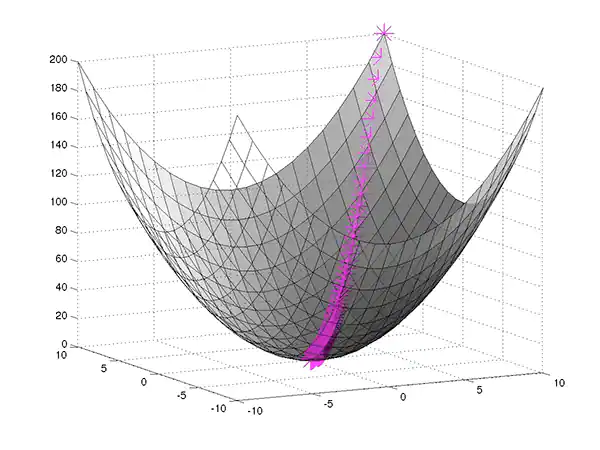
\includegraphics[width=100mm]{img/gdpic.png}
  \caption[]%
  {Gradient descent on 3D convex function [\url{https://www.digikey.be/nl/articles/get-started-machine-learning-hardware-and-software}].}
  \label{fig:gdp}
\end{figure}

\subsection{General gradient descent algorithm}
This section outlines the iterative process of calculating gradient descent for the objective function (MSE) we aim to minimize:

\begin{enumerate}
  \item \textbf{Compute gradient.}
  Calculate the first order partial derivative of the cost function with respect to each of the parameters.
  \item \textbf{Step in the opposite direction} 
  Subtract the gradient scaled by learning rate from parameter value.
  \item \textbf{Repeat until stop condition} Repeat the process until preset stop condition (or one of multiple) is reached.
\end{enumerate}

When we extend the example from \cref{Unmixing example}.
   We need to compute the gradient of the error function specific to our example from \cref{eq:err_gd_spec} in order to obtain the slope of tangent touching the error function with respect to the given parameter.
  \begin{equation}
  \frac{\partial}{\partial x_i} C(x)=\frac{\partial}{\partial x_i}\frac{1}{2D}\sum_{j=1}^{D}(\sum_{i=1}^{f}(x_iM_{i,j})-y_j)^2 
  \label{eq:err_gd_spec}
  \end{equation}
Substituting in:
  \[\begin{aligned}
  \frac{\partial}{\partial x_i} C(x)=\frac{\partial}{\partial x_i}\frac{1}{2D}(&(x_1 M_{1,1}+x_2 M_{2,1}-y_1)^2\\
  +&(x_1 M_{1,2}+x_2 M_{2,2}-y_2)^2\\
  +&(x_1 M_{1,3}+\alpha_2 M_{2,3}-y_3)^2)
 \end{aligned}\]

 If we take the partial derivative with respect to $x_1$ (partial derivative with respect to $x_2$ can be computed analogically):

  \[\begin{aligned}
  \frac{\partial}{\partial x_1} C(x)=&M_{1,1}(x_1 M_{1,1}+x_2 M_{2,1}-y_1)\\
  +&M_{1,2}(x_1 M_{1,2}+x_2 M_{2,2}-y_2)\\
  +&M_{1,3}(x_1 M_{1,3}+x_2 M_{2,3}-y_3)
 \end{aligned}\]
 Let us assume that from previous parameter update our current abundances are $x_1=0.9$ and $x_2=2$. We can now compute the gradient (analogically for $x_2$):
  \[\begin{aligned}
  \frac{\partial}{\partial x_1} C(x,t)=&1(0.9 \cdot 1+2 \cdot 2-7)\\
  +&2(0.9 \cdot 2+2 \cdot 1-5)\\
  +&3(0.9 \cdot 3+2 \cdot 1-6)\\
  =&-8.4
 \end{aligned}\]
  Next we use the the computed gradient for parameter update: \cref{eq:gd_update}. By subtracting the gradient we are stepping against it and therefore towards the minimum of the cost function.
 \begin{equation}
 x_i(t+1)=x_i(t)-\alpha\frac{\partial}{\partial x_i} C(x,t)
 \label{eq:gd_update}
  \end{equation}

 In \cref{eq:gd_update} $x_i(t)$ represents new value for the i-th abundance at current iteration, while $x_i(t)$ is the value from previous iteration. Finally $\alpha$ is the learning rate - a scaling factor (usually $\alpha<<1$) for the step size which needs to be set appropriately --- this means not too high so that gradient descent algorithm is able to converge to the minimum, and not too low in order for convergence to happen in reasonable time.
 
 Gradient from our example is negative which results in parameter increment. The increment magnitude will depend on learning rate and gradient size.
 
 We repeat the parameter update until we reach a predefined stop condition. While in an ideal world this would be 0 gradient (which corresponds to 0 sum of residuals), in real world this unlikely to ever happen. This is why we selected maximum number of iterations as our stop condition.
 
 However our example is idealized and we should be able to reach $100\%$ accurate abundances via a reasonable number of gradient descent iterations. When this happens and we recalculate the gradient with abundances $x_1=1$ and $x_2=3$:

  \[\begin{aligned}
  \frac{\partial}{\partial x_1} C(x,t)=&1(1 \cdot 1+3 \cdot 2-7)\\
  +&2(1 \cdot 2+3 \cdot 1-5)\\
  +&3(1\cdot 3+3 \cdot 1-6)\\
  =&0
 \end{aligned}\]
Indeed the gradient is 0 as expected. 


\subsection{Gradient descent variants implemented in Nougad}
Nougad is a library designed for the purpose of spectral unmixing, efficiently implemented in $C$ programming language with $R$ language interface \footnote{\url{https://github.com/exaexa/nougad}}. 
\subsubsection{Nougad variation on momentum method}
Momentum-based modification of the gradient descent algorithm "remembers" the previous update and allows it to increase the magnitude of the current update if they are both moving in the same direction. An acceleration factor is introduced to scale the influence of the previous update.

\begin{algorithm}
\caption{Nougad parameter update}
\label{algo:ngd_moment}
\begin{algorithmic}
\State $it \gets 0$
\While{$true$}
    \If{$up_i(t-1)\frac{\partial}{\partial x_i} C(x,t) > 0$} 
        \State $up_i(t) = \gamma up_i(t-1)+\frac{\partial}{\partial x_i} C(x,t)$
    \Else
        \State $up_i(t) = \frac{\partial}{\partial x_i} C(x,t)$
    \EndIf 

    \State $x_i(t) = x_i(t-1)+\alpha up_i(t)$
    \State $it = it+1$
    \If{$it \geq maxit$}
        \State $break$
    \EndIf 
\EndWhile
\end{algorithmic}
\end{algorithm}


In \cref{algo:ngd_moment} $\gamma$ represents the acceleration parameter while $up_i(t)$ is the update for $i$-th parameter in time $t$ and $maxit$ the number of iterations after which the algorithm stops.

Nougad also adds three options that are important in the context of spectral unmixing. 
\begin{enumerate}
    \item \emph{Contribution of negative abundances. - \param{nw}}
    
    This option sets a scaling factor for the contribution of negative spectral abundances to the update.
    Since we know that negative spectral abundances are impossible this parameter allows us to set a bias against such results.
    \item \emph{Contribution of positive/negative residuals - \param{spw}/\param{snw}}
    
    This option allows us to set a factor by which positive and negative residuals contribute to gradient, allowing us to set a preference for either positive or negative residuals and magnitude of their influence.
    \item \emph{Starting abundances - \param{start}}
    
    This option allows us to set a starting position for all abundances. Instead of starting at 0 we can potentially start at a number closer to a median value of the real abundances and hypothetically decrease the number of iterations needed to reach a solid result.
\end{enumerate}

Note that weighting the residuals and spectral abundances using \param{spw}, \param{snw} and \param{nw} is not considered in this pseudo-code to make it more concise however, it is a simple multiplication by a scalar. This implementation further allows us to explicitly set all other parameters used in gradient descent calculation including learning rate \param{alpha ($\alpha$)}, acceleration factor \param{accel ($\gamma$)} and a number of iterations \param{maxit}.

\subsubsection{Adam version of Nougad}
Adam stands for Adaptive Moment Estimation. The method computes the update based on moving averages of both the gradient itself (first moment) and its square (second moment), each with its own acceleration factor. 

\begin{equation}
\begin{aligned}
m_a(x_i,t) &= \beta_1 m_a(x_i,t-1)+(1-\beta_1)\nabla_iC(x)\\
m_s(x_i,t) &= \beta_2 m_s(x_i,t-1)+(1-\beta_2)\nabla_i^2C(x)\\
x_i(t) &= x_i(t-1)+\alpha \frac{m_a(x_i,t)}{\sqrt{m_s(x_i,t)}+\epsilon}
\end{aligned}
\label{eq:adam}
\end{equation}



In \cref{eq:adam} \param{b1 ($\beta_1$)} and \param{b2 ($\beta_2$)} are acceleration factors for first and second moment moving averages and $\epsilon$ is a very small scalar (usually $\leq 10^{-6}$) needed to avoid division by zero.

Options to emphasize influence of negative spectra abundances and positive/negative residuals are kept from the first method. All parameters including desired maximum number of iterations can again be passed as function arguments.
\subsection{Performance and acceleration of nougad}
Base implementation of nougad runs on CPU and is only single-threaded and while is inherently much slower than OLS it is still fast enough for an odd unmixing task. However, for any optimization/testing effort that requires hundreds or thousands of runs on large datasets (such as this thesis) a more performant implementation is desirable.

Luckily, since results of nougad for each cell are completely independent on other cells it lends itself very well to parallelization efforts. Simply put we can split cells into batches depending on core count and process them in parallel. In C we can even leverage pointers to avoid copying any of the large matrices as at no point should two threads process the same element.

A potential parallelized version therefore promises vast (and most likely near-linear) increase in performance for multi-threaded CPUs and potentially even higher performance for a version leveraging modern GPUs.  


